\documentclass[11pt]{article}
\usepackage[margin=1in]{geometry}
\usepackage{graphicx}
\usepackage{hyperref}
\usepackage{float}
\usepackage{tabularx}
\usepackage{booktabs}
\usepackage{array}

\hypersetup{colorlinks=true, linkcolor=blue, urlcolor=blue}
\setlength{\parskip}{0.45em}
\setlength{\parindent}{0pt}

\title{Software Requirements Specification\\MycoAI Retrieval System}
\author{MycoAI Project}
\date{May 19, 2026}

\begin{document}
\maketitle
\tableofcontents
\newpage

\section{Introduction}

This Software Requirements Specification defines the current MycoAI retrieval system. The system helps authenticated users upload fungal strain images, segment colonies, retrieve likely species, and view ranked results. Data owners additionally manage species data, index new strain images, review feedback, trigger training, and manage users.

\section{Actors}

\begin{table}[H]
\centering
\begin{tabularx}{\textwidth}{>{\raggedright\arraybackslash}p{3.5cm}X}
\toprule
Actor & Responsibilities \\
\midrule
Normal User & Authenticate, upload strain images, retrieve species, view results, and submit feedback. \\
Data Owner & Perform all Normal User actions, index new data, manage species and strains, review feedback, trigger training, view audit logs, and manage users. \\
AI Segmentation Service & Automatically detects colony regions from uploaded strain images. \\
Retrieval Service & Extracts features, searches vector data, aggregates neighbors, and returns ranked species results. \\
\bottomrule
\end{tabularx}
\end{table}

\section{Use Case Diagram}

\begin{figure}[H]
\centering
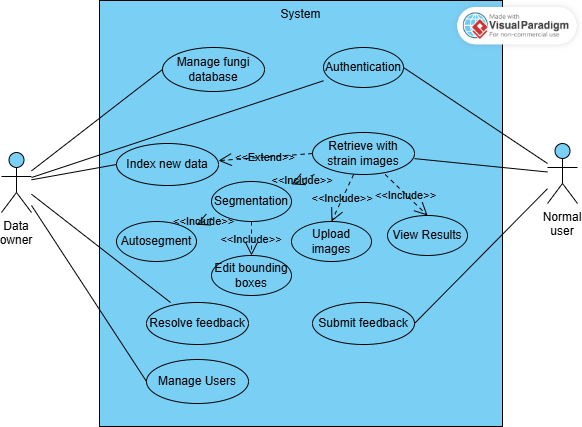
\includegraphics[width=0.95\textwidth]{assets/use-case-diagram.png}
\caption{MycoAI use case diagram.}
\label{fig:use_case_diagram}
\end{figure}

\section{Functional Requirements}

\subsection{Authentication}

\begin{enumerate}
  \item The system shall allow users to register with email, password, and name.
  \item The system shall allow users to log in and receive an authenticated session.
  \item The system shall require authentication for retrieval, data indexing, feedback, data management, training, and user management workflows.
  \item The system shall enforce role-based permissions for Normal User and Data Owner actions.
\end{enumerate}

\subsection{Retrieve Species}

Retrieve Species is the primary classification workflow for Normal Users and Data Owners.

\begin{enumerate}
  \item The system shall allow authenticated users to upload one or more strain images.
  \item The system shall collect strain identifier and growth medium metadata for each uploaded image.
  \item The system shall segment uploaded strain images before retrieval.
  \item The system shall allow users to view ranked species results with confidence scores.
\end{enumerate}

\subsection{Segmentation}

Segmentation is included by Retrieve Species.

\begin{enumerate}
  \item The system shall automatically segment colonies using AI.
  \item The system shall display detected bounding boxes over source images.
  \item The system shall allow users to edit bounding boxes before retrieval.
  \item The system shall generate colony crops for retrieval from accepted bounding boxes.
\end{enumerate}

\subsection{Index New Data}

Index New Data is a Data Owner use case that extends Retrieve Species.

\begin{enumerate}
  \item The system shall allow Data Owners to upload strain images for known species.
  \item The system shall reuse upload, segmentation, bounding-box editing, and result review from Retrieve Species.
  \item The system shall allow Data Owners to assign known species labels before indexing.
  \item The system shall index accepted colony segments so future retrieval can use the new data.
\end{enumerate}

\subsection{Other Data Owner Use Cases}

\begin{enumerate}
  \item The system shall allow Data Owners to create, read, update, archive, restore, and delete species, strains, images, and media records.
  \item The system shall allow Data Owners to review feedback and accept or reject proposed corrections.
  \item The system shall allow Data Owners to trigger and observe training or re-indexing jobs.
  \item The system shall allow Data Owners to manage user roles while preserving at least one Data Owner.
\end{enumerate}

\section{Nonfunctional Requirements}

\begin{enumerate}
  \item The system shall return single-image retrieval results within 5 seconds under normal operating conditions.
  \item The system shall protect data-modifying operations with authentication and role checks.
  \item The system shall preserve uploaded images, segmentation metadata, retrieval results, and audit-relevant changes.
  \item The system shall present workflows clearly for desktop research usage.
\end{enumerate}

\end{document}
